\documentclass[a4paper]{article}
\usepackage[utf8]{inputenc}
\usepackage{caption}
\usepackage{subcaption}
\usepackage[spanish]{babel}
\usepackage{graphicx}
\usepackage{xcolor}
\usepackage{amsmath}
\usepackage{hyperref}
\usepackage{todonotes}
\usepackage{biblatex}

\newcommand\imgScale {0.6}

\addbibresource{biblio.bib}

\title{Proyecto visión avanzada}
\author{Raúl Candela Arias \\ Francisco Morillas Espejo}
\date{Abril 2021}

\begin{document}

\maketitle

\section{Introducción}

El objetivo de este proyecto es el entrenamiento de redes convolucionales para realizar \textbf{segmentación semántica} de imágenes para detectar diferentes clases dentro de esta.
\newline

La segmentación semántica consiste en, dada una imagen, identificar a que clase de elemento corresponde cada píxel de esta.
Para ello, se crea una máscara de las mismas dimensiones que la imagen de entrada donde previamente se han coloreado las distintas clases (objetos) que se desean identificar (figura~\ref{fig:semanticSeg}).
\newline

La imagen original y la máscara se relacionan tal que, sea $A$ la imagen de entrada y $M$ la máscara, para cada píxel de la imagen $A_{i,j}$ tenemos que $M_{i,j} = c(A,i,j)$, donde $c$ es una función que indica a que clase pertenece el píxel ubicado en la imagen $A$ en la posición $i,j$.
\begin{figure}[htbp]
    \centering
    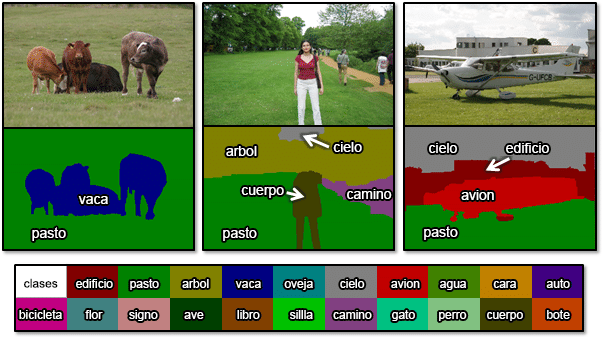
\includegraphics[scale=\imgScale]{img/EjSegSem.png}
    \caption{\small Ejemplo de segmentación semántica. \cite{Ref1}}
    \label{fig:semanticSeg}
\end{figure}

\section{Estado del arte}
A lo largo de la literatura se encuentran diferentes métodos para el reconocimiento de objetos a nivel de píxel, todos ellos haciendo uso de \textit{machine learning}~\cite{fabaret, long} pero, al unir series de convoluciones junto con capas de \textit{max-pooling} plantean problemas en la recreaci\'on de la imagen.
\newline

Por ello, Bradrinarayanan et al.~\cite{encoderDecoder} plantean una aproximaci\'on basada en arquitectura \textit{encoder-decoder}, solventando este problema y con unos resultados considerablemente superiores al resto.
En la figura~\ref{fig:segnet} se puede observar la arquitectura planteada.
\newline

Plantean una estructura en la que las capas del \textit{encoder} y del \textit{decoder} son sim\'etricas.
Las operaciones de \textit{upsamplig} del \textit{decoder} usan los \'indices de la capa correspondiente de \textit{max-pooling} del \textit{encoder}.
No hacen uso de conexiones residuales~\cite{resnet}.
\newline

Otra aproximaci\'on al problema es la planteada por Ronneberger et al.~\cite{unet} donde plantean una arquitectura \textit{encoder-decoder} llamada UNet (figura~\ref{fig:unet} en la que mediante salto de conexiones o conexiones residuales se concatena la \'ultima capa de convoluci\'on de la parte del \textit{encoder} con la primera capa de su correspondiente deconvoluci\'on en el \textit{decoder}, generando una forma de u.
Por su forma la parte del \textit{encoder} y del \textit{decoder} son sim\'etricas.
\newline

Como red de base a las arquitecturas mencionadas previamente en ocasiones se emplean modelos de redes ya existentes y pre-entrenados para grandes conjuntos de datos como ImageNet~\cite{imagenet} o COCO~\cite{coco}.
Entre estas se pueden destacar algunas como ResNet~\cite{resnet}, Xception~\cite{xception} o VGG-16~\cite{vgg} que destacan entre las m\'as comunes.

\begin{figure}[hbtp]
    \centering
    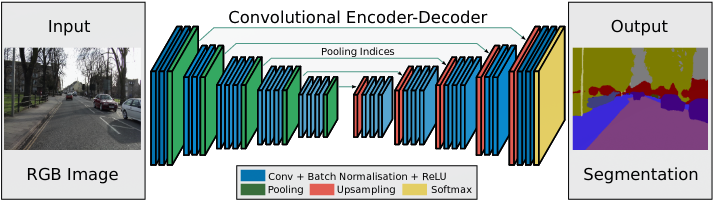
\includegraphics[scale=0.5]{img/segnet.png}
    \caption{\small Arquitectura SegNet.}
    \label{fig:segnet}
\end{figure}

\begin{figure}[hbtp]
    \centering
    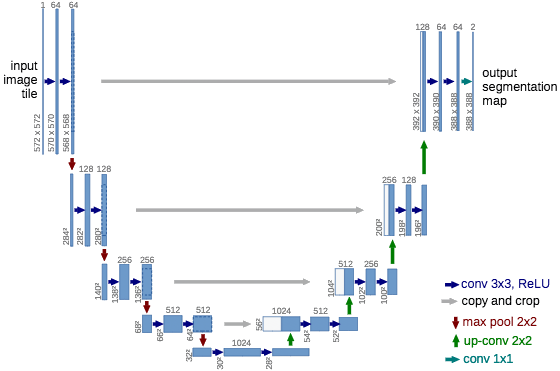
\includegraphics[scale=\imgScale]{img/unet.png}
    \caption{\small Arquitectura UNet.}
    \label{fig:unet}
\end{figure}
%A partir de esta idea, el modelo ded \textit{encoder-decoder} es el empleado en este campo de la visi\'on artificial.
%Aunque se distinguen diferentes arquitecturas para las dos partes.
%Dentro de las diferentes aproximaciones para la tarea de clasificación semántica se encuentra el modelo de \textit{encoder-decoder} como el más empleado.
%\newline

%En este tipo de modelos se recibe la imagen original como entrada y se pasa por una serie de capas convolucionales para extraer sus características aunque, como consecuencia la imagen reduce su tamaño.
%Tras esto se pasa por una serie de capas de deconvolución cuya salida proporcionará la máscara semántica de la imagen en cuestión.

\section{Desarrollo}
Para la implementación de la red se ha empleado una arquitectura UNet basada en el modelo Xception mediante la creaci\'on de una subclase de tipo \texttt{Model} dentro de la API de \texttt{Keras}.
\newline
    
La arquitectura presenta un modelo \textit{encoder-decoder} con cuatro tama\~nos de filtros diferentes, 32, 64, 128 y 256, tanto para las capas convolucionales como para las deconvoluciones. Estas capas son intercaladas con otras de \textit{Max Pooling} y de \textit{Up Sampling} dependiendo de si está en la parte del \textit{encoder} o en la del \textit{decoder}, así como con capas de \textit{Batch Normalization} y de \textit{Activation} independientemente de la ubicación.
\newline

Adem\'as, como se usa un modelo de red Xception se hace uso de capas convolucionales separables en profundidad (figura~\ref{fig:xception}).
Este tipo de convoluci\'on se caracteriza por estar construida por una convoluci\'on puntiaguda (\textit{depthwise convolution}) seguida de una profunda (\textit{pointwise convolution}).
\begin{itemize}
    \item Una convoluci\'on profunda es una convoluci\'on de n$x$n separada en canales. Por ejemplo, en el caso de haber 3 canales  se tendr\'ian 3 convoluciones de n$x$n.
    \item Una convoluci\'on puntiaguda es una convoluci\'on 1$x$1 usada para cambiar la dimensi\'on.
\end{itemize}

\begin{figure}[hbtp]
    \centering
    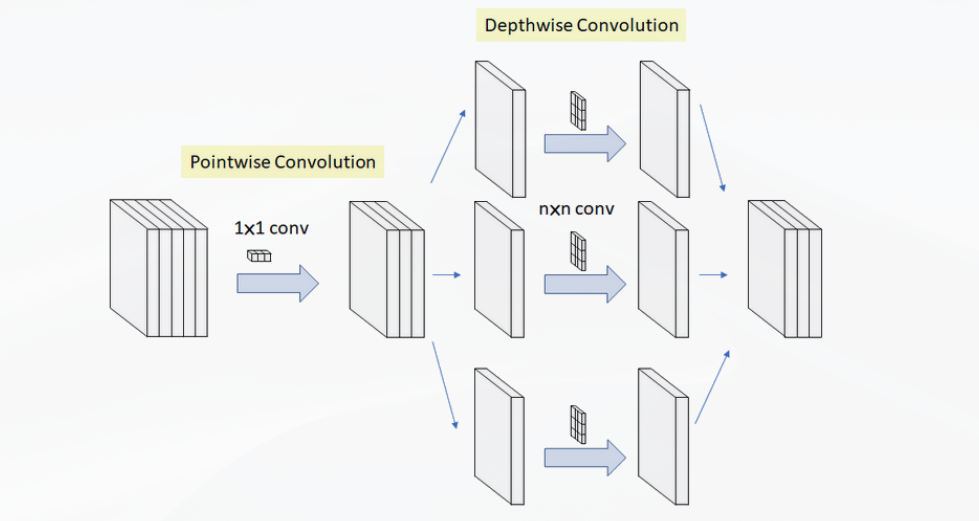
\includegraphics[scale=0.4]{img/xception.png}
    \caption{\small Convoluciones separables en profundidad utilizadas por Xception.}
    \label{fig:xception}
\end{figure}

Al seguir una estructura \textit{UNet} se realizan saltos entre las capas finales de las convoluciones (parte del \textit{encoder}) y las capas iniciales de las deconvoluciones (parte del \textit{decoder}).
\newline


Inicialmente se ha optado por realizar la segmentaci\'on sem\'antica en un conjunto de datos capturado con un dron llamado \textit{Semantic Drone Dataset}~\cite{droneDataset} el cual consta de 24 clases entre las que se distinguen personas, diferentes terrenos y objetos comunes que se pueden encontrar con una vista a\'erea.
\newline

Para ello se han cargado las distintas im\'agenes para los datos y las etiquetas con su correspondiente problem\'atica (ver secci\'on~\ref{subsec:cargaDataset}).
Se han convertido las etiquetas del espacio RGB a una matriz donde cada valor de color ahora se corresponde con un valor entero con una de las 24 posibles clases con el fin de mejorar el entrenamiento de la red.
Todo el sistema sea ha entrenado con la arquitectura mencionada previamente.
\newline

Como se menciona con m\'as detalle en la secci\'on~\ref{subsec:cambioDataset} se ha visto necesario cambiar a un \textit{dataset} m\'as peque\~no, en este caso se ha usado \textit{The Oxford-IIIT Pet Dataset}~\cite{petDataset}.
Este consiste en un conjunto de 37 categor\'ias de perros y gatos asociados a su m\'ascara para realizar la segmentaci\'on sem\'antica.
La estructura empleada para el entrenamiento es la misma que con el conjunto de datos anterior.


\section{Problemas encontrados}
\subsection{Creación la clase UNetX}
A la hora de crear el modelo se optó por realizarlo heredando de la clase \texttt{Model} de la API de \texttt{Keras}, lo cual ocasionó problemas debido a la falta de ejemplos de redes convolucionales complejas realizadas de este modo.
\newline

Una vez solventado, el m\'etodo de generar el modelo mediante herencia proporciona una mayor flexibilidad en cuanto al tipo de conexiones a realizar entre las capas, la posibilidad de generar diferentes modelos con distintos filtros o con una entrada de diferente tama\~no a lo largo del c\'odigo sin tener que crear nuevas funciones para cada caso.


\subsection{Carga del dataset \textit{Semantic Drone}}~\label{subsec:cargaDataset}
A la hora de realizar la carga del dataset hubieron varios problemas, entre ellos el formato de carga de las imágenes, la necesidad de procesar las etiquetas y la velocidad de carga de estas.\newline

En cuanto al formato, se empezó cargándolas con \textit{OpenCV} y reescal\'andolas a un tamaño de 480p, pero las imágenes eran demasiado grandes y finalmente se optó por realizar la carga con un tamaño de 224x224.\newline

Con respecto al procesado de las etiquetas, estas venían en formato \textit{.png} y debían ser reescaladas al mismo tamaño que la imagen original y convertirlas de una imagen con 3 canales a una matriz con las id de las etiquetas en cada píxel. Esta última conversión era excesivamente lenta y se intentó tanto realizarla en C como utilizar \texttt{numba} para intentar acelerarlo. Siendo esta la opción definitiva escogida.\newline

Finalmente se optó por utilizar el formato de imágenes de \texttt{PIL} y cargarlas con los métodos de \texttt{keras.preprocessing.image}.

\subsection{Cambio de dataset}~\label{subsec:cambioDataset}
Debido al gran tamaño de las imágenes originales del \textit{dataset} de \textit{Sematinc Drone} (4000 $x$ 6000), se optó por cambiar a un conjunto de datos con unas imágenes más pequeñas.
\newline

La problemática asociada al tamaño de las imágenes deriva directamente en el tamaño de la red.
Al ser imposible trabajar con las imágenes en su resolución original debido a la memoria VRAM necesaria hay que redimensionarlas a valores más aceptables dentro de las limitaciones físicas presentes, en este caso se ha visto que el valor que mejores resultados producía era de (224 $x$ 224) siendo este un valor inviable para este \textit{dataset} ya que la pérdida de información es demasiado grande.
\newline

Además, aún siendo un conjunto de datos muy pesado el número de imágenes es pequeño (400) por tanto es necesario aplicar métodos de \textit{data augmentation} tanto a las imágenes como a las etiquetas.
Por todo ello se ha optado por cambiar a un \textit{dataset} que se ajuste mejor.
\newline

El nuevo conjunto de datos posee un número más elevado de imágenes (7000), por lo que en principio no es necesario aumentarlo, y la resolución de las imágenes es bastante variada pero se sitúa entre los 200 y 500 píxeles, por lo tanto no supone ningún problema trabajar con una resolución de 224 $x$ 224.


\newpage
\section{Resultados}
A continuación se pueden observar los resultados obtenidos tras el entrenamiento de la red (ver figura~\ref{fig:prediction}), así como la imagen de origen y la máscara que se ha usado para entrenar la red (ver figuras~\ref{fig:origImg} y~\ref{fig:groundTruth}).
\newline

En las figuras~\ref{fig:acc} y~\ref{fig:loss} se puede ver las gráficas obtenidas en uno de los múltiples entrenamientos realizados.
Se puede observar como, al tratarse de un problema sencillo el sistema sobreentrena como bastante facilidad.
\newline

Para mejorar la calidad de la máscara de salida se podría realizar un postprocesado de ésta con técnicas de visión convencional, por ejemplo realizando operaciones morfológicas de apertura y cierre.

\begin{figure}[hbtp]
    \centering
    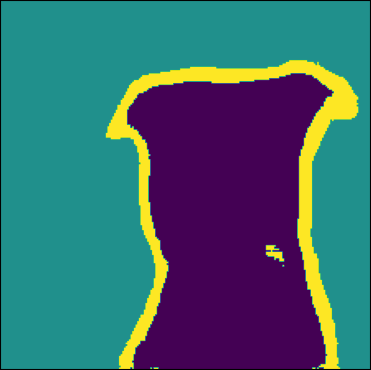
\includegraphics[scale=\imgScale]{img/prediction.png}
    \caption{\small Predicci\'on de la m\'ascara generada por la red.}
    \label{fig:prediction}
\end{figure}
\begin{figure}[hbtp]
    \centering
    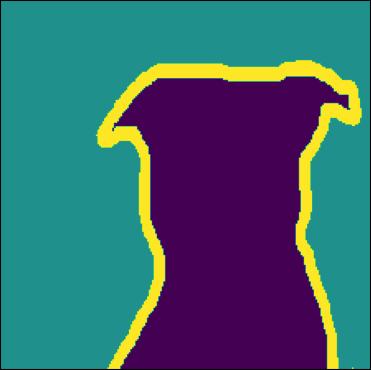
\includegraphics[scale=\imgScale]{img/groundTruth.png}
    \caption{\small \textit{Ground truth} de la imagen.}
    \label{fig:groundTruth}
\end{figure}
\begin{figure}[hbtp]
    \centering
    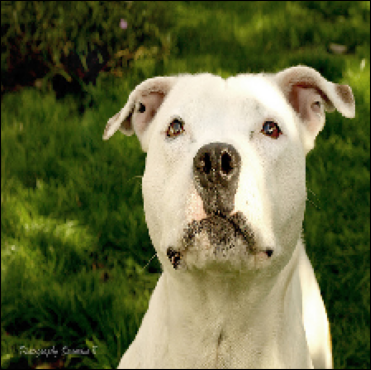
\includegraphics[scale=\imgScale]{img/originalImg.png}
    \caption{\small Imagen sin m\'ascara.}
    \label{fig:origImg}
\end{figure}

\begin{figure}[hbtp]
    \centering
    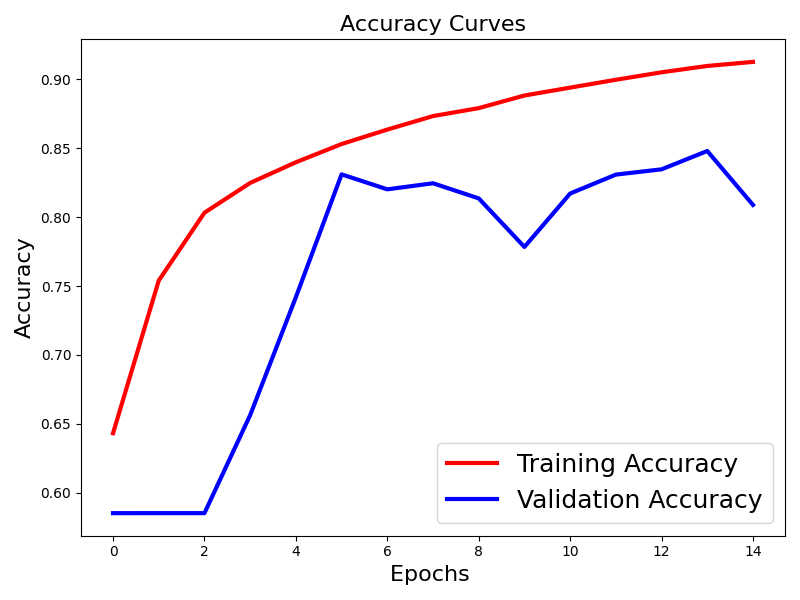
\includegraphics[scale=\imgScale]{img/accs.png}
    \caption{\small Curvas de precisión de la red.}
    \label{fig:acc}
\end{figure}
\begin{figure}[hbtp]
    \centering
    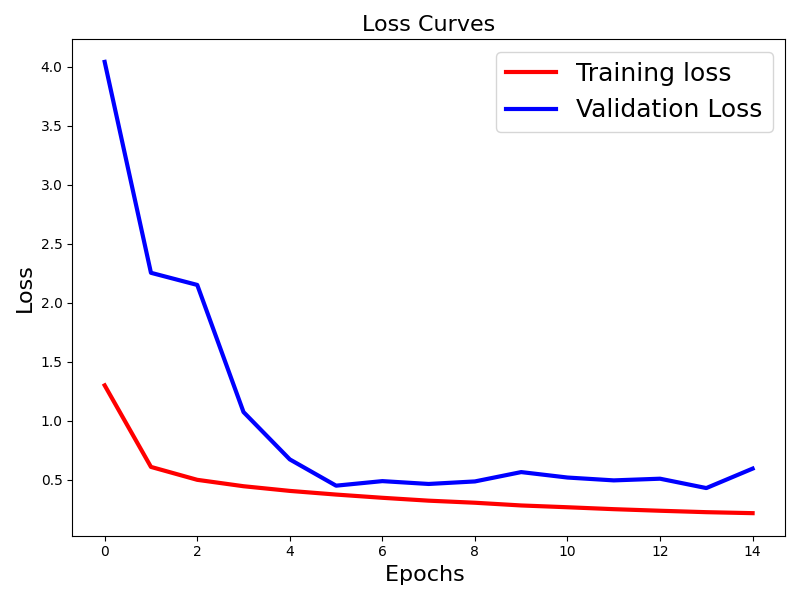
\includegraphics[scale=\imgScale]{img/losses.png}   
    \caption{\small Curvas de pérdida de la red.}
    \label{fig:loss}
\end{figure}
\section{Conclusiones}
En este proyecto se ha podido observar como por medio de modelo basado en un autoencoder se ha realizado una segmentación semántica de perros y gatos que distingue entre:
\begin{enumerate}
    \item Animal
    \item Borde
    \item No animal
\end{enumerate}

Se ha visto que es una aproximación muy simple y que da buenos resultados con una baja cantidad de etiquetas a diferenciar además de tener un entrenamiento muy rápido.\newline

También se han podido observar algunos problemas, como que debido a usar capas convolucionales separables, la cantidad de memoria utilizada sube bastante, haciendo que sea difícil de entrenar si se escala la red.\newline

Como futuro trabajo se podría probar a aumentar el número de clases a detectar, haciendo que no solo distinga entre animal, borde y no animal; sino entre animales también.

\newpage
\printbibliography
\end{document}
